\chapter{Background Information}

Consistent with the nature of robotics, the work presented herein draws on concepts from multiple differing fields. This chapter serves to provide background information to familiarize the reader with some of the fundamental information used to achieve the goal of intent estimation. 

\section{Models of locomotion}

Modeling gait walking is one of the main components of gait velocity estimation and it may be achieved using simple physics-based template models. Physics-based models may be actuated or passive i.e., without any control inputs.  

\subsection{Actuated Models}

One approach to gait modeling is including a control input to achieve the desired gait. An example of this approach is the Variable-SLIP (V-SLIP) model, which utilizes variable stiffness actuation to modulate leg stiffness in contrast to the original B-SLIP model that has constant leg stiffness~\cite{visser2017bipedal}. This model produces a gait that is robust to disturbances, and whose cost of transport is comparable to human walking\footnote{Cost of transport quantifies the energy efficiency of a system, it measures the energy expended to travel a specified distance.}. Another approach is to vary the CoM height by applying a force along the leg~\cite{koolen2016balance}. While all the previously described models have nonlinear dynamics, Kajita et al.~\cite{kajita1991study} proposed a model called the Linear Inverted Pendulum (LIP) model in which the application of a constraint control input linearizes the dynamics of the system. The LIP model also allows the use of ankle torques to improve model performance on rugged terrain. The LIP model has been extended to three dimensions with the 3D-LIP model~\cite{kajita20013d}.

Actuated models provide a more flexible framework to estimate gait, but determining the control parameters when applying those models to humans becomes a challenge. Therefore, active models are more suited to legged robots or prosthetic devices which are used in series with the user. The simplicity of passive models and the ability to modify the initial conditions to accommodate the effects of a user working in parallel makes them more suited for parallel robots such as exoskeletons. Most active models have been proposed in regards to legged robots where the dynamics of the robot are well known to the designers. This allows for the complexity of the model to be matched to the complexity of the system dynamics. With the case of exoskeletons, the dynamics of the human body are still a subject of study and they are further complicated by the parallel operation with the exoskeleton suit due to coupling in the human and robot. As a result, passive models may be better suited for use in intent detection frameworks due to their relative simplicity.

\subsection{Passive Models}

It has been shown that passive models can accurately generate gaits that qualitatively resemble key features of human locomotion~\cite{mochon1980ballistic}. The most basic passive model is an inverted pendulum (IP) with the center of mass (CoM) vaulting over a stiff leg. However, it was observed that animal gaits exhibit significant energy storage in muscles, tendons, and ligaments. As a result, legged locomotion may be analogous to a spring-mass system~\cite{blickhan1989spring} with the CoM loaded onto a compliant leg, modeled as a spring. This characterization of legged locomotion could not be reconciled with the stiff leg utilized in the IP model and a new model, called the Spring-Loaded Inverted Pendulum (SLIP), was proposed to add compliance to the leg via a massless spring~\cite{blickhan1989spring}. It has been observed that relative leg stiffness of animals ranging from dogs and rams to humans and kangaroos is similar during running~\cite{blickhan1993similarity} and that the CoM falls to its lowest position at midstance across species, compressing a virtual spring and releasing that stored energy as the gait progresses~\cite{full1999templates}. This dynamic similarity can be further reinforced using the Froude numbers for various animals. The Froude number is a metric that non-dimensionalizes velocity with leg length and gravity. Multi-legged animals exhibit gait transitions at similar Froude numbers, suggesting that may be possible to use template models to capture gaits for a more generalized set of subjects with respect to their morphology.

The SLIP model can be used to describe human running, however, it is inadequate to describe human walking. The IP model exhibited CoM trajectories with higher vertical oscillation than observed in human trials for both walking and running~\cite{lee1998determinants}. The discrepancy in the CoM trajectories was found to increase with forward velocity. The IP and SLIP models lack the double support phase, which is crucial during walking. These deficiencies were addressed when Geyer proposed an extension of the SLIP model, called the Bipedal-SLIP (B-SLIP) model, in which the CoM is supported by two massless springs of fixed stiffness~\cite{geyer2006compliant}. The  B-SLIP model matches human CoM trajectories and ground reaction force (GRF) profiles, at average walking and running velocities. Thus the B-SLIP model is a unified model that can exhibit multiple gaits across a range of velocities. While the B-SLIP model addresses the shortcomings of IP and SLIP models, it has its drawbacks when walking at extreme velocities. The model exhibits oscillations during the double support phase at low velocities in the range of walking speeds exhibited by individuals with SCIs. These oscillations may be the result of the 2D nature of these models.

In their basic forms, the IP, SLIP and B-SLIP models all ignore lateral dynamics, however, lateral dynamics become more dominant for low-speed gaits. For example, according to the human walking data presented by Fukuchi et al.~\cite{fukuchi2018public}, the peak-to-peak amplitude of the lateral sway of the CoM is approximately 3 cm while walking at 1.27 m/s but it rises to 9 cm while walking at 0.44 m/s. The model presented by Geyer is defined in only two dimensions, but it generalizes to 3D~\cite{liu2015dynamic}. This 3D model allows the lateral sway to be taken into consideration and oscillations during double support are eliminated. With appropriate leg length and step width, the sway seen in the gaits generated using the 3D B-SLIP model is comparable to human data. Taking the lateral sway into consideration is especially important while studying walking at low speeds. 

\section{The B-SLIP model}
The work presented herein is focused on individuals recovering from iSCIs whose walking velocities were as low as 0.4 m/s. A majority of the the duration of steps at low velocities is spent in double support, and it is important to use a model than can describe this gait phase. Therefore, this work considers the 3D B-SLIP model to model human locomotion shown in Fig~\ref{fig:slip}. In this model, the \COM is loaded onto two massless spring legs of length $ l_o $ and stiffness $ k $. The position and velocity of the point mass $ m $ are given by $ \p_{\COM} = [x_{\COM} ,y_{\COM} ,z_{\COM}]^T $ and $ \v_{\COM} = [v_x ,v_y ,v_z]^T $. The position of the leading leg at touchdown is given by two angles, the angle between the leading leg and vertical $ \theta $ and the angle $ \varphi $ between the forward axis $ x $  and the ground projection of the leading leg.

\begin{figure}
	\centering
	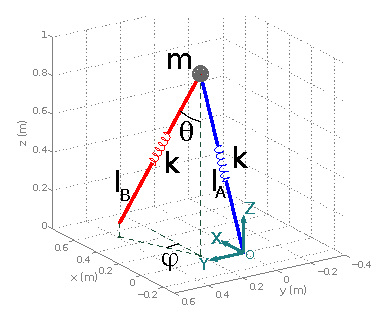
\includegraphics[width=0.6\linewidth]{3DSLIP.eps}
	\caption{The Bipedal Spring Loaded Inverted Pendulum \cite{liu2015dynamic} model of walking}\label{fig:slip}
\end{figure}

\begin{figure}
	\centering
	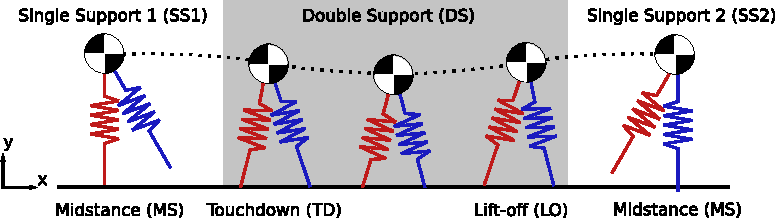
\includegraphics[width=\linewidth]{slip_gait.pdf}
	\caption{One step of a B-SLIP gait}\label{fig:slip_gait}
\end{figure} 

A gait of the B-SLIP model, as viewed in the sagittal plane \footnote{The saggital plane is the plane that divides the body into right and left parts.}, is illustrated in Fig.~\ref{fig:slip_gait}. This gait starts at midstance (MS), where the CoM is loaded onto the trailing leg in single-support (SS1). The gait then proceeds with the touchdown (TD) of the leading leg and enters the double support (DS) phase. The DS phase ends with lift-off (LO) of the trailing leg and the model enters the second single-support phase (SS2). The SS2 phase ends in MS, again with the CoM loaded onto the leading leg. As there are alternating SS and DS phases, the dynamics of the B-SLIP model are hybrid.

\subsection{Hybrid dynamics of the B-SLIP model}
The dynamics of the model in single support are described by
\begin{equation}
	m\ddot{\p_{\COM}} = k(l_0 - \lVert \mathbf{l}_i \rVert)\hat{\mathbf{l}}_i + m \mathbf{g}
\end{equation}
\noindent where $ i = \{A,B\} $ denotes the supporting leg, $ \mathbf{l}_i \in \mathbb{R}^3 $ is the vector along the leg from the mass to the position of the stance foot $\p_i$ , $ \hat{\mathbf{l}}_i \in \mathbb{R}^3$ is a unit vector along the leg, and $ \mathbf{g} \in \mathbb{R}^3 $ is the gravity vector. The dynamics during double support are given by
\begin{equation}
	m\ddot{\p_{\COM}} = k(l_0 - \lVert \mathbf{l}_A \rVert)\hat{\mathbf{l}}_A + k(l_0 - \lVert \mathbf{l}_B \rVert)\hat{\mathbf{l}}_B + m \mathbf{g}
\end{equation}

\noindent Certain conditions, known as guards, must be met to enable the switching of the dynamics from one phase to another. There are three switching surfaces to enable phase switches at TD, LO, and MS. These sets are as follows

\begin{eqnarray}
	\mathcal{G}_{TD} &=& \{(\p,\v)| v_z < 0 ,z_{\COM} < z_{T}\} \\
	\mathcal{G}_{LO} &=& \{(\p,\v)| v_z > 0 ,\lVert \mathbf{l}_A \rVert > l_0\} \\
	\mathcal{G}_{MS} &=& \{(\p,\v)| v_z = 0 ,z_{\COM} > z_{T} ,\lVert \mathbf{l}_A \rVert < l_0\} 
\end{eqnarray} 

\noindent where $ z_{T} = l_0 \cos \theta $ is the threshold height for touchdown. Satisfaction of these guard conditions triggers gait phase switches and the states of the model are transferred across the switching events using functions called reset maps. There are three reset maps for the B-SLIP model following the general form $ \x^+ = \mathcal{R(\x^-)} $, where the $ + $ and $ - $ denote pre- and post-switch states. One map is applied at TD and the other at LO such that

\begin{eqnarray}
	\mathcal{R}_{TD}:\x^- &\rightarrowtail& I\x^- :\mathbb{R}^6 \rightarrowtail \mathbb{R}^6 \\
	\mathcal{R}_{LO}:\x^- &\rightarrowtail& I\x^- ,\p_B \leftarrow \p_A :\mathbb{R}^6 \rightarrowtail \mathbb{R}^6 \\
	\mathcal{R}_{MS}:\x^- &\rightarrowtail& I\x^- :\mathbb{R}^6 \rightarrowtail \mathbb{R}^6
\end{eqnarray}

The are not impacts at touchdown as spring legs of the B-SLIP model are assumed to be massless. Reset maps handle touchdown impacts for models that consider the mass of the feet. Thus, the B-SLIP model can exhibit periodic gaits by alternately switching through SS and DS phases.

As the B-SLIP model is passive, it does not have any active control inputs to modify gaits and maintain periodicity. Therefore, optimization methods need to be used to find periodic model gaits as steady-state human walking is periodic. Poincar\'e maps are used in the gait optimization \cite{strogatz2018nonlinear,garcia1998simplest} to find periodic gaits.

\section{Poincar\'e maps}

\begin{figure}
	\centering
	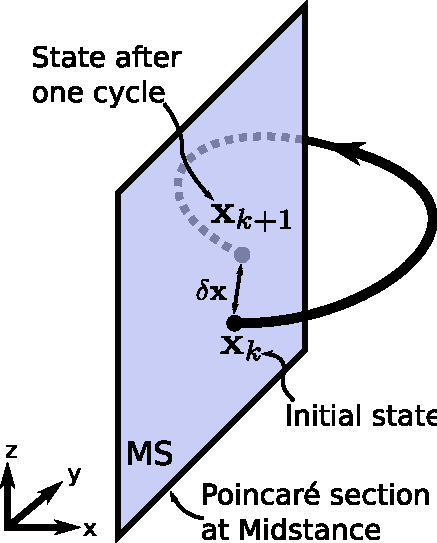
\includegraphics[width=.25\linewidth]{poincare.pdf}
	\caption{A Poincar\'e map used to find periodic gaits}\label{fig:poincare}
\end{figure}

A Poincar\'e section for a dynamical is a subspace that has fewer dimensions that the model's state space. It may be placed at a gait event such as MS, TD, or LO when the value of one of the states may be fixed e.g., when the vertical velocity of the \COM is zero. Let the Poincar\'e section be placed at MS, and let $ \mathcal{P} $ of the state $ \x_k $ be a function that returns the state after one cycle, or a step in the case of the B-SLIP, such that $ \x_{k+1} = \mathcal{P}(\x_k) $. The function $ \mathcal{P}(\x_k) $ is the Poincar\'e map and there exists an initial state representing a periodic orbit where the initial state maps back to itself after one period such that $ \x_k = \mathcal{P}(\x_k) $.
%
%\begin{equation}
%	\x_k = \mathcal{P}(\x_k)
%\end{equation}
%

A Poincar\'e section placed at MS is shown in blue in Fig.~\ref{fig:poincare}. The dynamics of the model are integrated for one step using $ \x_k $ as the initial condition. Optimization methods are used to find initial conditions that yield periodic gait by minimizing $ \delta \x $, the error between $ \x_k $ and $ \x_{k+1} $. The nonlinear return map may be linearized about these periodic gaits for further refining the gait search as described in Chapter \ref{chapter:IMM}. Model gaits for various velocities may be used as references while estimating an exoskeleton user's desired gait. Measurements of quantities such as CoM height and velocity, may be compared to simulated model gaits using state estimation tools such as the Kalman filter. 

\section{State estimation using Kalman filters}

Kalman filtering is a feedback-based sequential optimal state estimation technique \cite{kalman1960new}. The optimality of this technique stems from the method of computing feedback gain that accounts for modeling and measurement errors. A fundamental assumption about the nature of these errors is that they are zero-mean Gaussian noise processes. The filter was originally proposed for discrete-time linear systems. 
 
\subsection{Discrete-time Kalman Filter}
The filter is initialized at a certain initial state estimate $ \hat{\x}_0 $ that may have associated uncertainty due to measurement errors. The evolution of this state is described using dynamical system presented in the following equations
%
\begin{eqnarray}
	\x_{k+1} &=& \A_k \x_k + \B_k \u_k + \mathbf{G} \mathbf{w}_k,\quad \mathbf{w}_k \sim \mathcal{N}(0, \Q_k) \label{eq:sys_disc}  \\
	\tilde{\y}_k &=& \H_k \x_k + \mathbf{v}_k,\quad \mathbf{v}_k \sim \mathcal{N}(0,\R_k) \label{eq:meas_lin}
\end{eqnarray}
%

\noindent where $ \x_k $ and $ \u_k $ are the discrete-time states and inputs, $ \y_k $ are the discrete-time measurements, $ \A_k $, $ \B_k $, $ \H_k $ are the system, input, and measurement models respectively. The system has zero-mean Gaussian noises for process noise $ \mathbf{w}_k $ and measurement noise $ \mathbf{v}_k $ with covariances  $ \Q_k $ and $ \R_k $ respectively. The measurement noise $ \mathbf{w}(t) $ is combined with the measurement equation $ \H_k \x_k$ to form the noisy measurement $ \tilde{\y}_k $. 

\begin{figure}
	\centering
	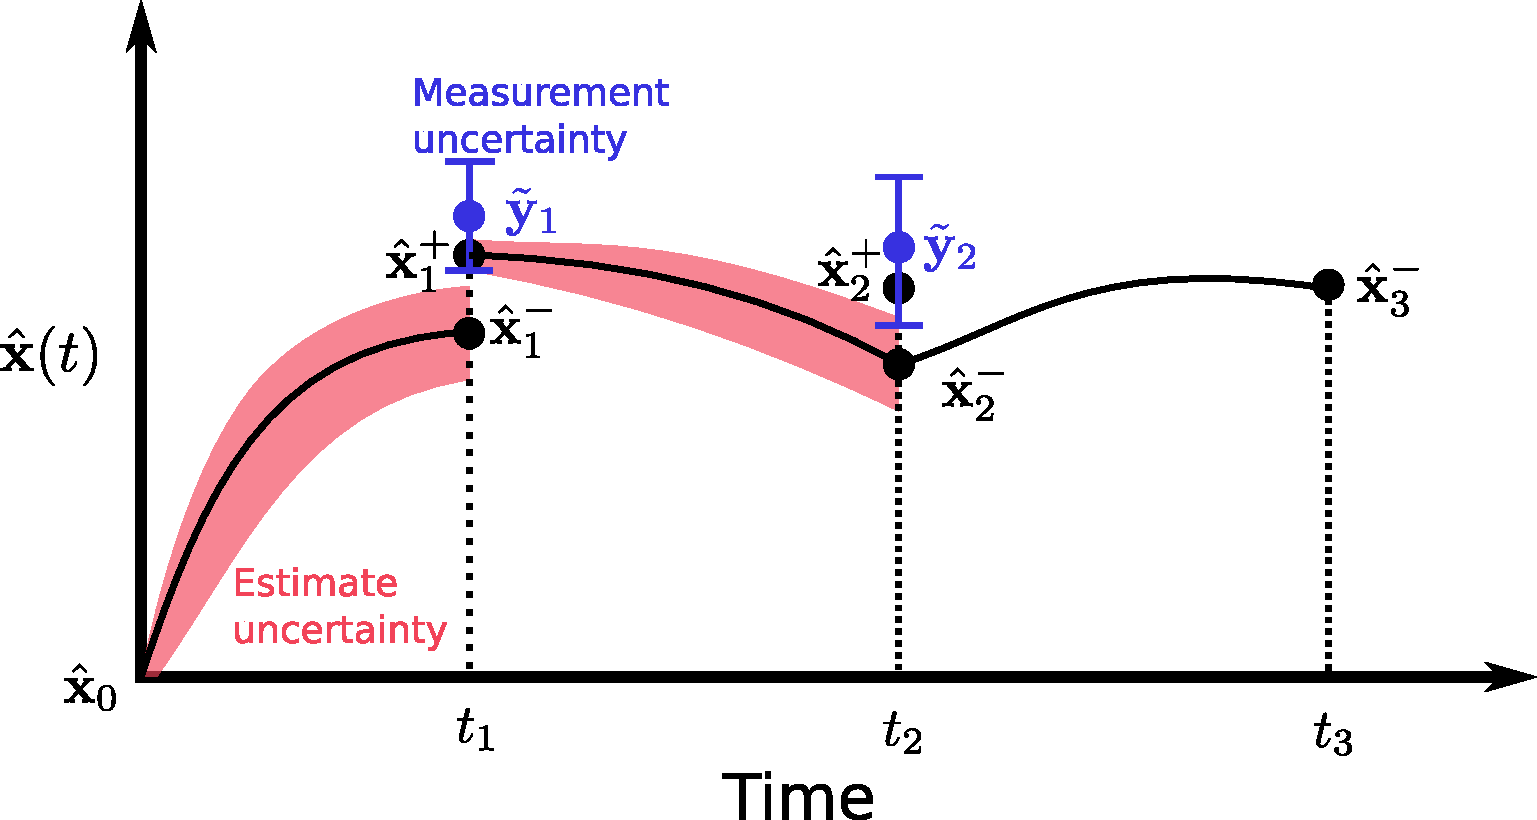
\includegraphics[width=0.7\linewidth]{kalman.pdf}
	\caption{Illustration of the Kalman Filtering process}\label{fig:kalman}
\end{figure}

The uncertainty associated with the estimates increases as the state is propagated forward through time using the system dynamics. Regular measurements of state variables are used to update the state estimates and reduce the uncertainty as illustrated in Fig.~\ref{fig:kalman} where the $ + $ and $ - $ in the superscript denote pre- and post-update states. The system illustrated here is discrete, however a continuous state evolution is shown to better illustrate the growth in uncertainty. Kalman filters account for both, the uncertainty in the state estimates and in the measurements. Further details of this process are as follow. The state estimates and estimate covariance $ \P $ are propagated in discrete time such that
\begin{eqnarray}
	\hat{\x}_{k+1} &=& \A_k \hat{\x}_k + \B_k \u_k \\
	\P_{k+1} &=& \A_k\P_k \A_k^T + \mathbf{G}_k\Q_k\mathbf{G}_k^T 
\end{eqnarray}
\noindent The states are sequentially updated such that
\begin{eqnarray}
	\K_k &=& \P_k^- \H^T_k \left[\H_k \P_k^- \H^T_k + \R_k\right]^{-1} \\
	\hat{\x}_k^+ &=& \hat{\x}_k^- + \K_k[\tilde{\y}_k- \H_k \hat{\x}_k^-)] \\
	\P_k^+ &=& [\mathbf{I} - \K_k \H_k]\P_k^-
\end{eqnarray}

\noindent where the updated estimates, their covariance and the Kalman gain are $ \mathbf{x}_k^+ $, $ \mathbf{P}_k^+ $, and $ \K_k $ respectively. The Kalman gain is optimal and the error dynamics of the filter are shown to be stable \cite{Crassidis} using the Lyapunov candidate function $ V(\e) = \e_k^T P_k^{-1} \e_k $ where $ \e_k \equiv \hat{\x}_k - \x_k $. The filter as described above is defined for linear systems, and it has been extended to nonlinear systems.

\subsection{Extended Kalman Filter}

Simple models used to describe legged locomotion have nonlinear dynamics and a variation of the Kalman filter named the Extended Kalman Filter (EKF) can be used for these systems. The nonlinear dynamics are linearized about the state estimate to work around the nonlinearity. As this linearization is an approximation of the dynamics, the EKF is not optimal like the discrete-time Kalman filter described previously. In spite of the lack of optimality, EKFs have been in widespread use for nonlinear systems. Since most nonlinear dynamics are given in continuous time, a variation of the EKF called the Continuous-Discrete EKF may be used. In this variation, dynamics evolve in continuous time, and measurements are modeled in discrete time. This combination is used for estimation in the work presented herein as it most closely reflects the model and measurement conditions observed in the estimation problem being studied. The general structure of the EKF is similar to the filter presented previously, except the equations are nonlinear as seen by comparing Eq. \eqref{eq:sys_disc} and \eqref{eq:sys}. Consider the following dynamical system with nonlinear dynamics
% Continuous-Discrete EKF
%
\begin{eqnarray}
	\dot{\x}(t) &=& \mathbf{f}(\x(t),\u(t),\mathbf{w}(t),t),\quad \mathbf{w}(t) \sim \mathcal{N}(0, \Q(t))  \label{eq:sys}  \\
	\tilde{\y}_k &=& \mathbf{h}(\x_k) + \mathbf{v}_k,\quad \mathbf{v}_k \sim \mathcal{N}(0,\R_k) \label{eq:meas}
\end{eqnarray}
%
\noindent where $ \x(t) $ and $ \u(t) $ are the continuous-time states and inputs, $ \y_k $ are the discrete-time measurements, and $ \mathbf{f}(\x(t),\u(t),t) $ and $ \mathbf{h}(\x_k) $ are the system and measurement function respectively. The system has zero-mean Gaussian process and measurement noises $ \mathbf{w}(t) $ and $ \mathbf{v}_k $ respectively with covariances $ \Q(t) $ and $ \R_k $ respectively. The measurement noise $ \mathbf{w}(t) $ is combined with the measurement equation $ \mathbf{h}(\x_k) $ to form the noisy measurement $ \tilde{\y}_k $. 

The state estimates and estimate covariance $ \P $ are propagated in continuous time such that
\begin{eqnarray}
	\dot{\hat{\x}} &=& \mathbf{f}(\hat{\x},\u,t) \\
	\dot{\P}(t) &=& \F(t)\P(t) + \P(t)\F^T(t) + \mathbf{G}(t)\Q(t)\mathbf{G}(t)^T \\ 
	\F(t) &\equiv& \frac{\partial \mathbf{f}}{\partial \x} \Bigr |_{\hat{\x}(t),\u(t)} \nonumber
\end{eqnarray}


\noindent The states are sequentially updated such that
\begin{eqnarray}
	\K_k &=& \P_k^- \H^T_k(\hat{\x}_k^-) \left[\H_k(\hat{\x}_k^-)\P_k^- \H^T_k(\hat{\x}_k^-) + \R_k\right]^{-1} \\
	\hat{\x}_k^+ &=& \hat{\x}_k^- + \K_k[\tilde{\y}_k-\mathbf{h}(\x_k)] \\
	\P_k^+ &=& [\mathbf{I} - \K_k \H_k(\hat{\x}_k^-)]\P_k^-,\quad \H_k(\hat{\x}_k^-) \equiv \frac{\partial \mathbf{h}}{\partial \x} \Bigr |_{\hat{\x}_k^-}
\end{eqnarray}

\noindent where $ \K_k $ is the Kalman gain, $ \F(t) $, and $ \H_k(\hat{\x}_k^-) $ are the linearized dynamics and measurement model respectively. The updated estimates and their covariance are $ \mathbf{x}_k^+ $ and $ \mathbf{P}_k^+ $ respectively. The above equations describe a Continous-Discrete Kalman filter setup. System dynamics are propagated in continuous time but states are updated in discrete time since measurements are discrete. This setup handles the nonlinear dynamics of the models used to emulate legged locomotion. Each step of human walking has alternating single and double support periods depending on how many legs are in contact with the ground. Therefore, addition to being nonlinear, models of legged locomotion have hybrid dynamics to describe different gait phases i.e., different dynamics for different phases. The EKF can be used as an estimation tool to handle these hybrid dynamics in a framework known as Interacting Multi-Model (IMM) estimation. This framework is used in Chapter~\ref{chapter:IMM} to estimate an exoskeleton user's gait speed and gait phase.